\begin{surferIntroPage}{Primeros pasos con SURFER}
Este programa se llama SURFER. Si le\'es esta palabra probablemente pienses que tiene algo que ver con el agua, el sol y las olas... pero no. El nombre viene del ingl\'es {\it surface}, que en espa\~nol significa {\it superficie}.\\
Con SURFER se pueden graficar superficies algebraicas. Lo que esto significa y lo que son las superficies algebraicas ser\'a explicado en este tutorial, que pod\'es empezar a recorrer eligiendo una de las superficies que est\'an a la derecha.\\
SURFER es parte de la exhibici\'on IMAGINARY, que empez\'o en el a\~no 2008 cuando Alemania decidi\'o celebrar su A\~no de la Matem\'atica. La exhibici\'on es un proyecto del mundialmente conocido Mathematisches Forschungsinstitut Oberwolfach situado en la Selva Negra alemana. Cada semana tienen lugar all\'i distintas reuniones sobre temas que se investigan en matem\'atica. Estas reuniones son importantes para fomentar el intercambio entre cient\'ificos en todo el mundo. \\
\vspace{0.2cm} \hspace{3.5cm}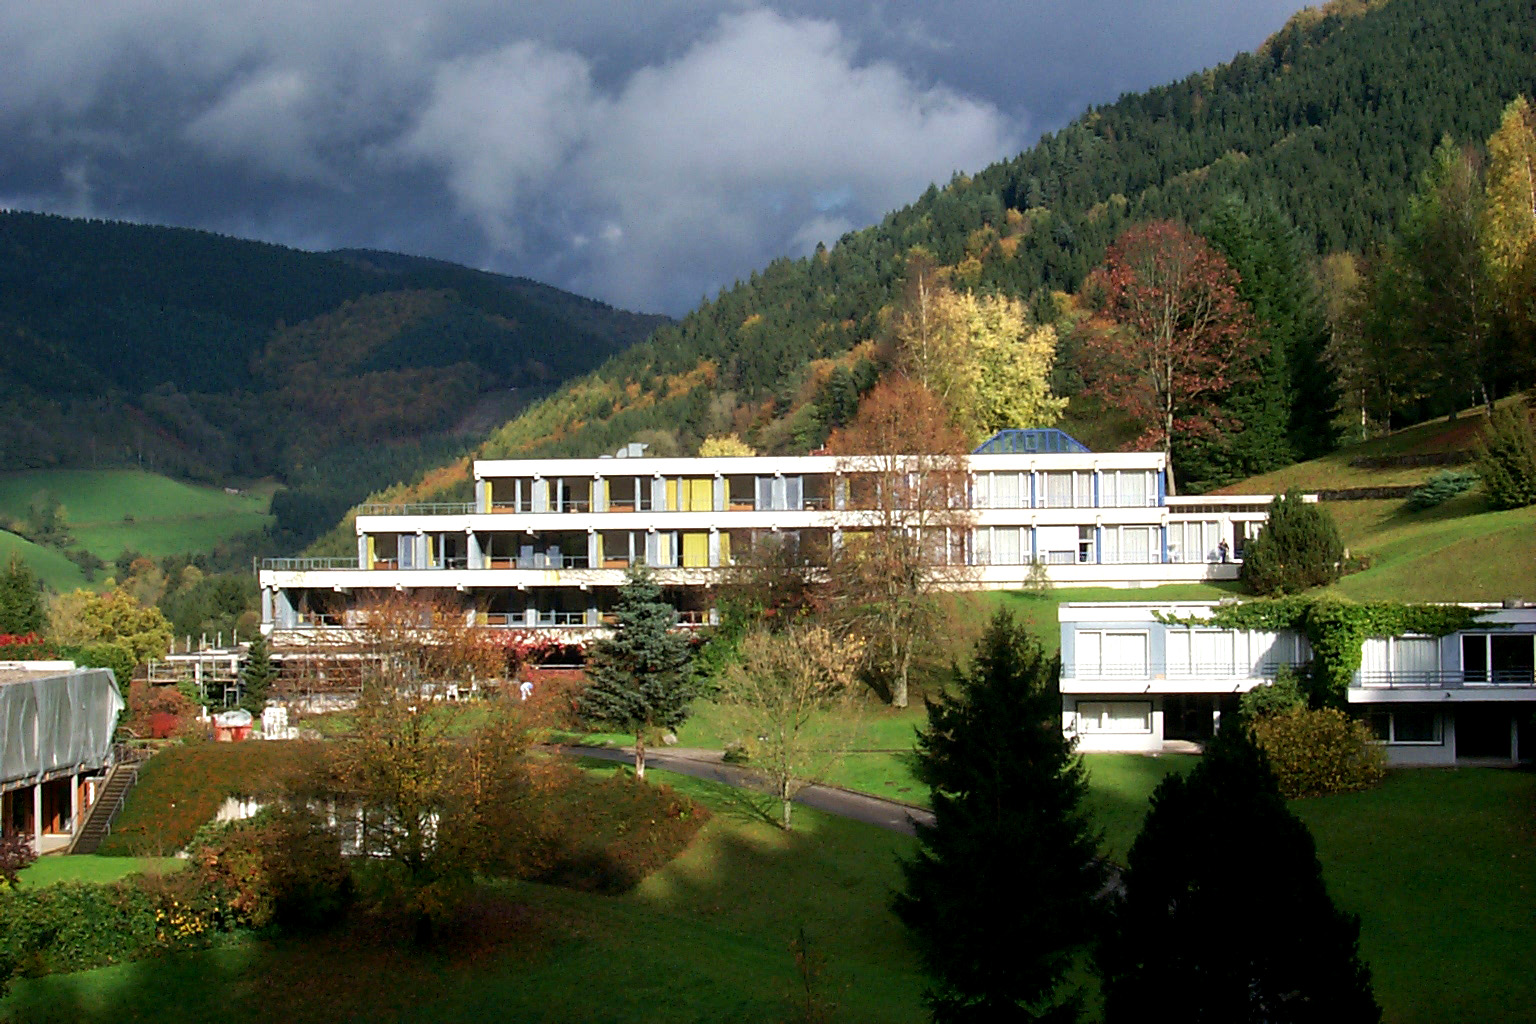
\includegraphics[width=3cm]{../../common/images/photo_mfo.jpg}\\
El programa SURFER puede ser descargado gratuitamente desde el sitio web \\
\begin{centering}
www.imaginary-exhibition.com\\
\end{centering}
 \vspace{0.2cm}
A la derecha pod\'es elegir alguno de los tutoriales, siendo el primero de estos el correspondiente a la superficie Lim\'on. A la izquierda pod\'es ir a otra galer\'ia, por ejemplo la de las superficies de fantas\'ia.
\end{surferIntroPage}